\documentclass[7pt]{beamer}
\usepackage{beamerthemesplit}
\usepackage{amsfonts}
\usepackage{amsmath}		
\usepackage{amssymb}
\usepackage{float}
\usepackage{graphicx}
\usepackage{longtable}
\usepackage{makeidx}
\usepackage{rotating}
\usepackage{wasysym}

%\usepackage[latin2]{inputenc}
%\usepackage[romanian,magyar]{babel}
\usepackage{graphicx}
%\usepackage{dsfont}
\usepackage{beamerthemesplit}
\usepackage{hyperref}
\definecolor{red}{RGB}{0,0,200}
\mode<presentation>
{
\newtheorem{dfn}{Definition}[section]
\newtheorem{lem}[dfn]{Lemma}
\newtheorem{thm}[dfn]{Theorem}
\newtheorem{prop}[dfn]{Proposition}
\newtheorem{rem}[dfn]{Remark}
\newtheorem{cor}[dfn]{Corollary}
\newtheorem{ex}[dfn]{Example}
\newtheorem{pf}[dfn]{Proof}
%\newtheorem{notn}[dfn]{Notation.}
\newcommand{\R}{\mathbb R}
\newcommand{\F}{\mathbb F}
\newcommand{\C}{\mathbb C}
\newcommand{\N}{\mathbb N}
\newcommand{\Z}{\mathbb Z}
\newcommand{\Q}{\mathbb Q}
\newenvironment{notn}[1][Notation]{\noindent\textbf{#1.} }{\ \rule{0.0em}{0.0em}}
%Defining Caligraphic letters
\newcommand{\calL}{\mathcal{L}}
\newcommand{\calN}{\mathcal{N}}
\newcommand{\calP}{\mathcal{P}}
\newcommand{\calB}{\mathcal{B}}
\newcommand{\calO}{\mathcal{O}}
\newcommand{\calK}{\mathcal{K}}
\newcommand{\calG}{\mathcal{G}}
\newcommand{\calD}{\mathcal{D}}
\newcommand{\calU}{\mathcal{U}}
\newcommand{\calR}{\mathcal{R}}
%\begin{comment}
\newcommand{\al}{\alpha}
\newcommand{\be}{\beta}
\newcommand{\ga}{\gamma}
\newcommand{\Ga}{\Gamma}
\newcommand{\te}{\theta}
\newcommand{\et}{\eta}
\newcommand{\om}{\omega}
\newcommand{\Om}{\Omega}
\newcommand{\ps}{\psi}
\newcommand{\Ps}{\Psi}
\newcommand{\daba}{\partial}
%\newcommand{\p}{\pi}
\newcommand{\ph}{\phi}
\newcommand{\de}{\delta}
\newcommand{\ro}{\rho}
\newcommand{\si}{\sigma}
\newcommand{\Si}{\Sigma}
\newcommand{\la}{\lambda}
%\newcommand{\m}{\mu\psi}
\newcommand{\vp}{\varphi}
\newcommand{\ep}{\varepsilon}
\newcommand{\id}{\,\mathrm{d}}




%\setbeamertemplate{itemize item}[ball]

  \useoutertheme{infolines}
  \usetheme[hideothersubsections]{Berkeley}
  \usecolortheme[named=red]{structure}
  \usecolortheme{whale}
  \useinnertheme{rounded}
  \usefonttheme[onlymath]{serif}
  \setbeamertemplate{blocks}[rounded][shadow=true]
  \setbeamertemplate{navigation symbols}{}
  \usecolortheme{sidebartab}
}
%======================================================================================
% SLIDE 1: TITLE
%======================================================================================

\title[Bathymetry Inversion from Waves]{Inverting for Near Coastal Bathymetry from Surface Wave Properties}
\author[USACE Bathymetry]{Presented \\ by\\Us\\Supervised by\\Ty  Hesser (USACE)\\Lea Jenkins (Clemson)}
\institute[IMSM]{Industrial Mathematical and Statistical Modeling}
\date{July 2016}
%\logo{\includegraphics[height=1.4cm,width=1.5cm]{aust_logo}}
\begin{document}
 \frame{\titlepage}
\frame{
\frametitle{}
\tableofcontents
}
\section{Introduction }
%==============================================================================================================================
%SLIDE 3: Bathymetry is topography under the sea
%======================================================================================

\begin{frame}
\frametitle{Bathymetry is topography under the sea}
It's important for things like

\begin{columns}
\column{0.5\textwidth}
\begin{itemize}
\item Marine navigation
\item Repairing of storm damage
\item Military planning
\end{itemize}
\column{0.5\textwidth}
\begin{figure}[h]
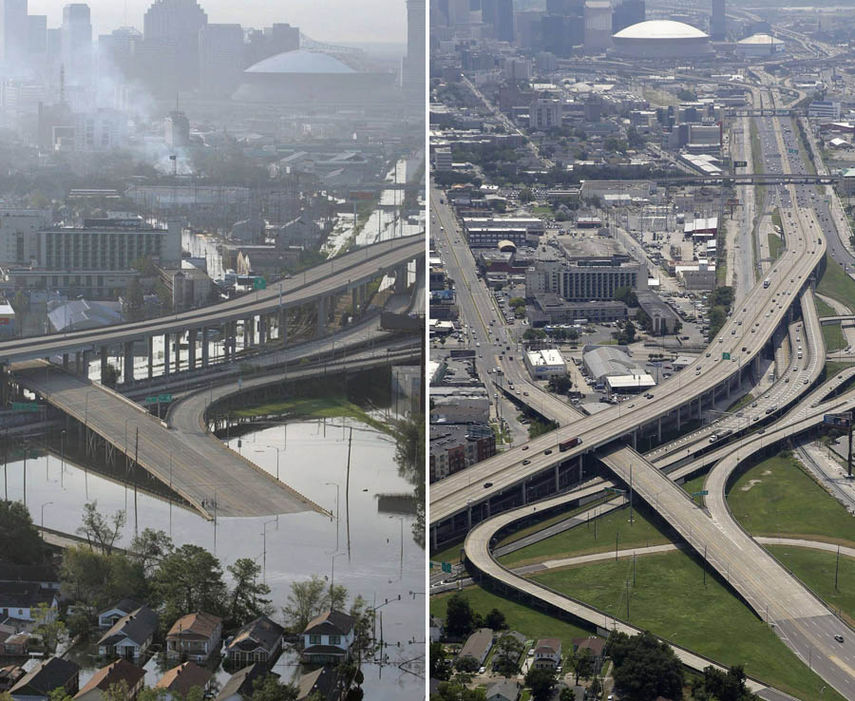
\includegraphics[width=.80\linewidth]{img/Flood_D.jpg}\hfill

\end{figure}

\end{columns}


%\begin{itemize}
%\item Marine navigation
%\item Repairing of storm damage
%\item Military planning
%\end{itemize}
%\begin{figure}[h]
%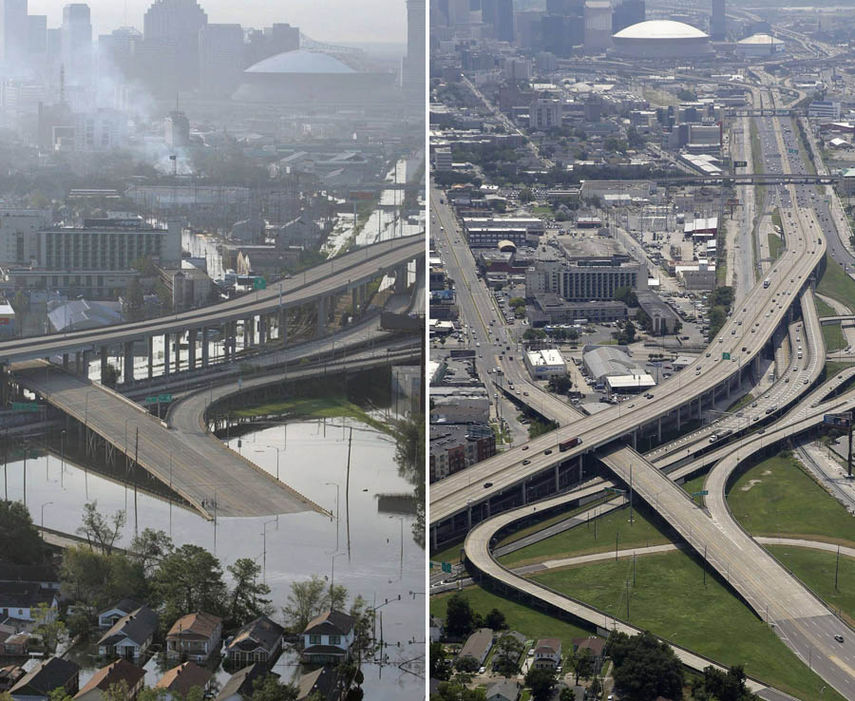
\includegraphics[width=.40\linewidth]{img/Flood_D.jpg}\hfill

%\end{figure}


\end{frame}
%==========================================================================================================================================
% SLIDE 4: Getting measurements of coastal bathymetry can be kind of lame
%======================================================================================

\begin{frame}
 \frametitle{Getting measurements of coastal bathymetry can be kind of lame}
 In situ bathymetry data is
 \begin{itemize}
 \item Expensive to collect
 \item Located in a hazardous environment (surf zone)
 \item Sparse in time and space
 \end{itemize}

\begin{figure}[h]
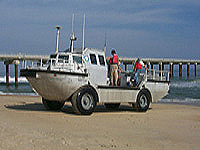
\includegraphics[width=.40\linewidth]{img/LARC.jpg}\hfill
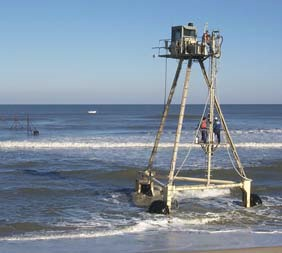
\includegraphics[width=.40\linewidth]{img/CRAB2.JPG}
\end{figure}
\end{frame}



%==========================================================================================================================================
% SLIDE 5: But we can invert for bathymetry given surface measurements
%======================================================================================

\begin{frame}
 \frametitle{But we can invert for bathymetry given surface measurements}

Our goal is to estimate bathymetry with surface wave data instead of direct measurements of the submarine environment

\begin{figure}[H]
	 	\centering
	 	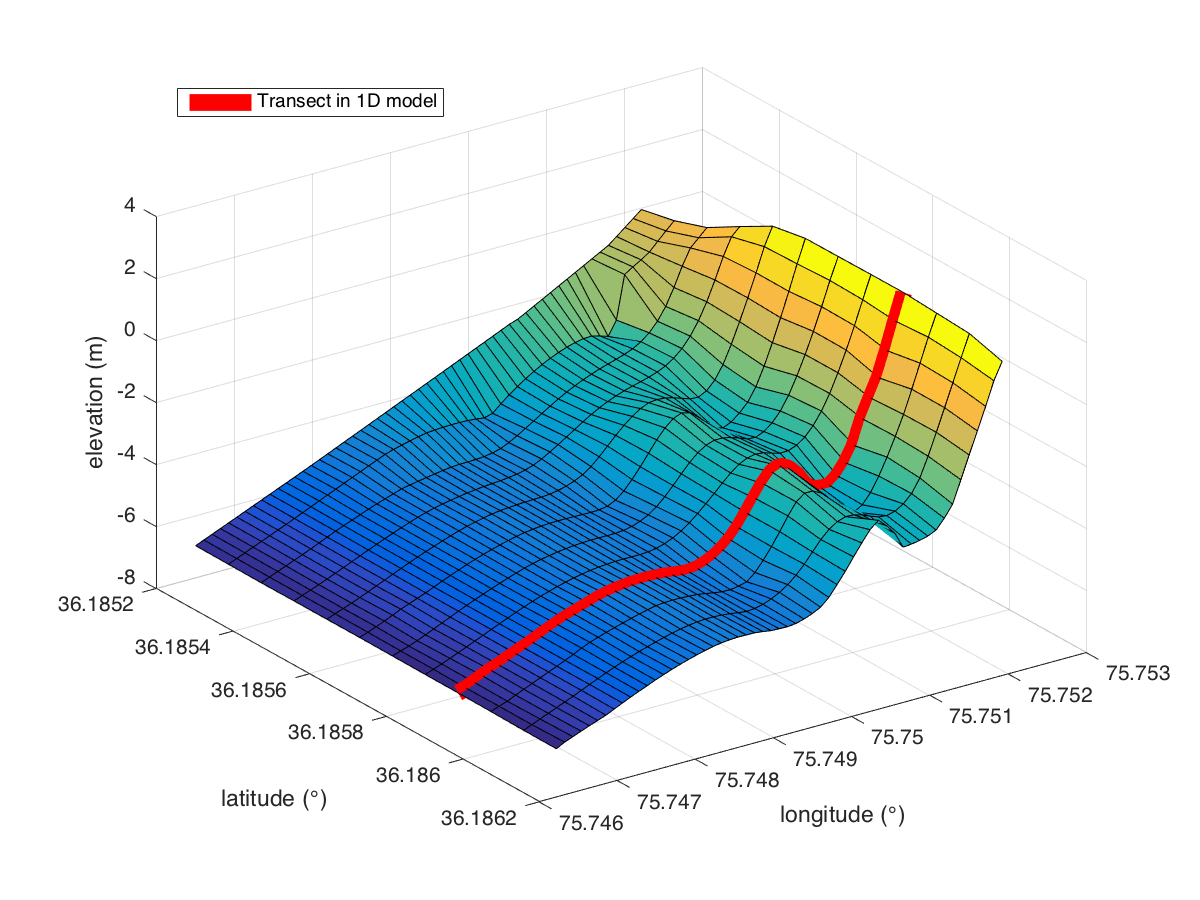
\includegraphics[width=0.6\linewidth]{img/trueBath2D.png}
	 	\caption{Measured and gridded 2D bathymetry in the survey area on 1 October 2015. The red line shows the transect considered in the 1D problem.}
	 	\label{2D Bath}
	 	\end{figure}

\end{frame}
%==========================================================================================================================================
\section{Methods}
%==========================================================================================================================================
% SLIDE 6: 1D wave physics is well known for near coastal regions
%======================================================================================
\begin{frame}
 \frametitle{1D wave physics is well known for near coastal regions}
\centering
\begin{itemize}
\item 1D Forward Model
\end{itemize}

\begin{eqnarray*}
\label{fp1}
\left \{
\begin{array}{lll}
\frac{d}{dx}\left(EC_g\right)=-\delta,\\
\\
\sigma^2=gk\tanh(kh),
\label{ode}
\end{array}
\right.
\end{eqnarray*}
\begin{flushleft}
where,
\end{flushleft}
$${E: Wave \,Energy,\, C_{g}: Group \,celerity,}$$
$${\quad c: Wave \,celerity,\, \sigma: Angular \,frequency,}$$
$${\quad\quad\quad\quad g: Gravitational\,\, acceleration,k: Wave \,number}$$
\end{frame}
%==========================================================================================================================================
% SLIDE 7: We have plenty of wave data...and some bathymetry
%======================================================================================

\begin{frame}
\frametitle{We have plenty of wave data...and some bathymetry}
\begin{columns}
\column{0.5\textwidth}
\begin{itemize}
\item Boundary Conditions (T,H)
\item Light Detection and Ranging(H)
\end{itemize}
\column{0.5\textwidth}
\begin{itemize}
\item CRAB/LARC (h)
\item Argus Video Monitioring (k,f)
\end{itemize}
\end{columns}

\begin{figure}[H]
\centering
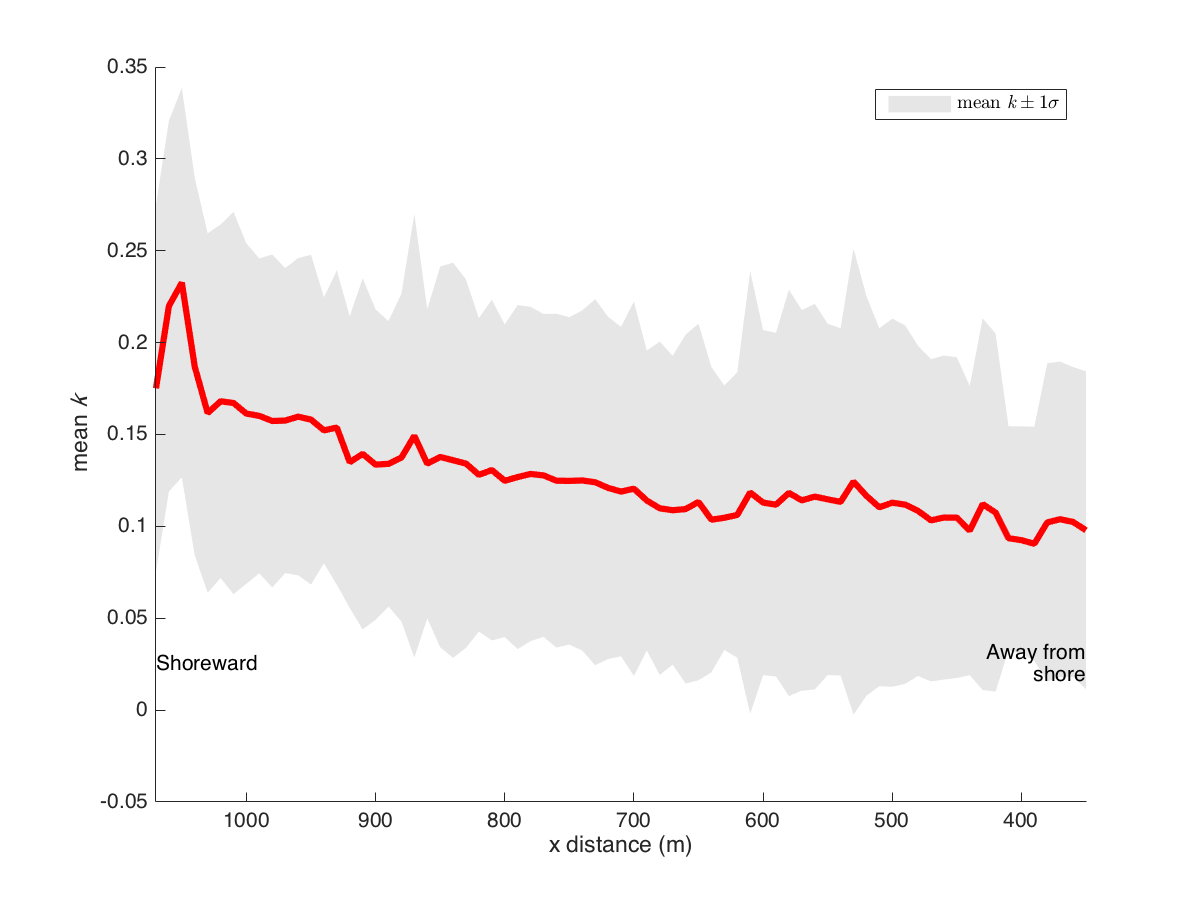
\includegraphics[width=.45\linewidth]{img/k1Dmean_std.png}
\caption{Argus- photogrammetry used to derive wave frequency and wave number.}

\end{figure}
\end{frame}

%==========================================================================================================================================
% SLIDE 8: We invert for bathymetry given the surface data and physics
%======================================================================================

\begin{frame}
 \frametitle{We invert for bathymetry given the surface data and physics}

\begin{itemize}
\item Least squares
\item MCMC
\item fmincon
\item etc.
\end{itemize}


\end{frame}
%==========================================================================================================================================
\section{Results}
%==========================================================================================================================================
% SLIDE 9: We tried several inverse methods
%======================================================================================

\begin{frame}
 \frametitle{We tried several inverse methods}
\begin{itemize}
\item Nonlinear least squares
\item MCMC
\item fmincon
\end{itemize}
\end{frame}
%==========================================================================================================================================

%==========================================================================================================================================
% SLIDE 10: Nonlinear least squares
%======================================================================================

 \begin{frame}
\frametitle{Nonlinear least squares}


\end{frame}


%==========================================================================================================================================
% SLIDE 11: Bayesian Markov Chain Monte Carlo (MCMC) Method
%======================================================================================

 \begin{frame}
\frametitle{Bayesian Markov Chain Monte Carlo (MCMC) Method}
The MCMC method was used to create a posterior distribution of depth profiles, given wave number by using the Bayes relationship

\begin{equation}\label{bayes}
P(h|%H,
k) \propto \Pi(h)L(h|%H,
k),
\end{equation} 
where $\Pi(h)$ is the prior distribution, $L(h|%H,
k)$ is the likelihood function, and $P(h|%H,
k)$ is the posterior distribution.
\end{frame}

%==========================================================================================================================================
% SLIDE 12: MCMC Method: Log-Likelihood Function
%======================================================================================
\begin{frame}
 \frametitle{MCMC Method: Log-Likelihood Function}
\begin{itemize}
\item The loglikelihood uses the sum of square errors between simulated and observed \textit{k} to quantify the probability that the modeled \textit{k} represents the true \textit{k} profile as observed.
\begin{equation} \label{likely}
\log{L(h|%H,
k)}=log{e^{- \frac{\sum\limits_{i=1}^n({k}_{m,i}-k_{d,i})^2}{2\sigma_{d}^2}}}
\end{equation} 

\end{itemize}
\end{frame}
%==========================================================================================================================================
% SLIDE 13: MCMC Method: Metropolis Algorithm

%==========================================================================================================================================
\begin{frame}
 \frametitle{MCMC Method: Metropolis Algorithm}
\begin{itemize}
\item The prior and likelihood are combined to compute an initial posterior probability distribution of \textit{h}\\
\begin{equation}\label{post}
P(h|%H,
k) = log(\Pi(h)) + log(L(h|%H,
k))
\end{equation}
\item The algorithm then uses a markov chain random walk to %propose and compare new \textit{h} profiles
arrive at a posterior distribution of \textit{h} profiles which are expected to describe true bathymetry
\end{itemize}
\end{frame}
%==========================================================================================================================================

%SLIDE 14: fmincon
%==========================================================================================================================================
 \begin{frame}
\frametitle{fmincon}


\end{frame}


%==========================================================================================================================================


%==========================================================================================================================================
%SLIDE 15: Future directions
\section{Discussion}
%==========================================================================================================================================
\begin{frame}
 \frametitle{Future directions}
 \begin{itemize}
 \item 2D problem
 \item Regularization methods
 \item Use of wave heights
 \item Other dominant modes of k (and f)
 \end{itemize}

\end{frame}
%========================================
% Slide 16: THANK YOU
%========================================
\begin{frame}
\frametitle{}
\hspace{2.5cm}
\begin{minipage}{50mm}   
                                                                                                                           
      \begin{alertblock}{}    
                                          
            \begin{center}
                                                                                                                                                                                  
                  \textbf{THANK YOU!}
                            
                                                                       
            \end{center}
      \end{alertblock}
\end{minipage}
\end{frame}
%===========================================================================================================================================


\end{document}

